\documentclass{article}

%% Page Margins %%
\usepackage{geometry}
\geometry{
    top = 0.75in,
    bottom = 0.75in,
    right = 0.75in,
    left = 0.75in,
}

\usepackage{amsmath}
\usepackage{graphicx}
\usepackage{parskip}

\title{Lab 5: Counters and Clocks}

% TODO: Enter your name
\author{Frederick Meneses}

\begin{document}
\maketitle

\section{Part I}

\begin{enumerate}
\item Export the subcircuit schematic as an image and include it in your report.

\begin{figure}[ht!]
    \centering
    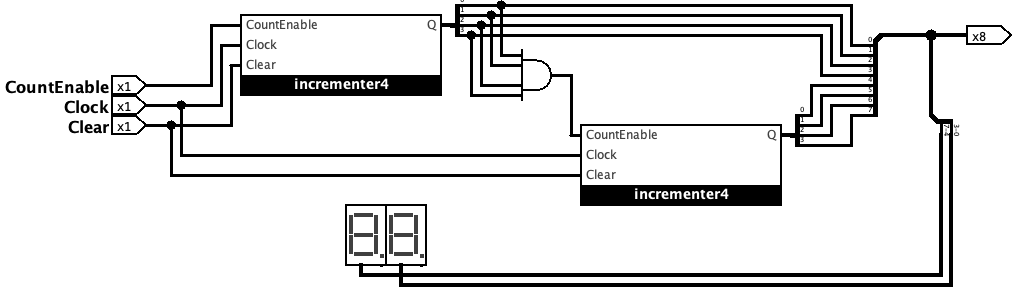
\includegraphics[width=0.65\textwidth]{lab5_counter8.png}
    \caption{A schematic of counter8.}
    \label{f:counter8}
\end{figure}

\item Include a screenshot of your simulation.
\begin{figure}[ht!]
    \centering
    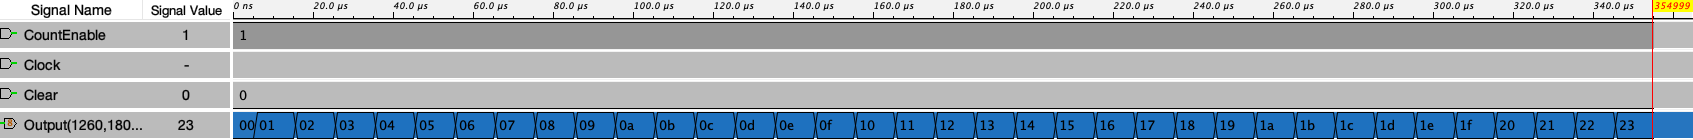
\includegraphics[width=0.65\textwidth]{lab5_counting8_timing.png}
    \caption{A timing diagram for counter8.}
    \label{f:counter8_timing}
\end{figure}

\end{enumerate}

\section{Part II}

\begin{enumerate}
\item The check for the maximum value is not necessary in the example above. Explain why in your prelab report.
It is not necessary because the CounterOut will rise to 1 when it hits the maximum value and reset the counter.

\item If you wanted this 4-bit counter to count from 0-9, how would you adjust the circuit above?
Add a comparator to the output of the counter where its output is connected to the input of the counter, comparing the counter's memory to the 4-bit value 1001, resetting the counter if it reaches 9.

\item In Properties there is a setting called Action On Overflow. Explain how each value for this setting responds to overflow by experimenting with this setting and describing the results. \\
Wrap around: if counting up, then the next value after overflow is 0. If counting down, then the next value after overflow is the maximum value.\\
Stay at value: At overflow, if counting up, then the counter stays at the maximum value. If counting down, then it stays at 0. They stay at this value until bit width is reached. After which, it stays at the loaded value until it continues. \\
Continue counting: At overflow, If counting up, then the counter's memory resets itself but keeps counting until it hits the maximum number of bit allotted. If counting down, then counts from the maximum until the maximum allotted bit is reached. Whatever is loaded in the bit input load, is saved for the next cycle. \\
Load next value: Loads the next value from the bit input load.

\item Export the subcircuit schematic as an image and include it in your report.

\begin{figure}[ht!]
    \centering
    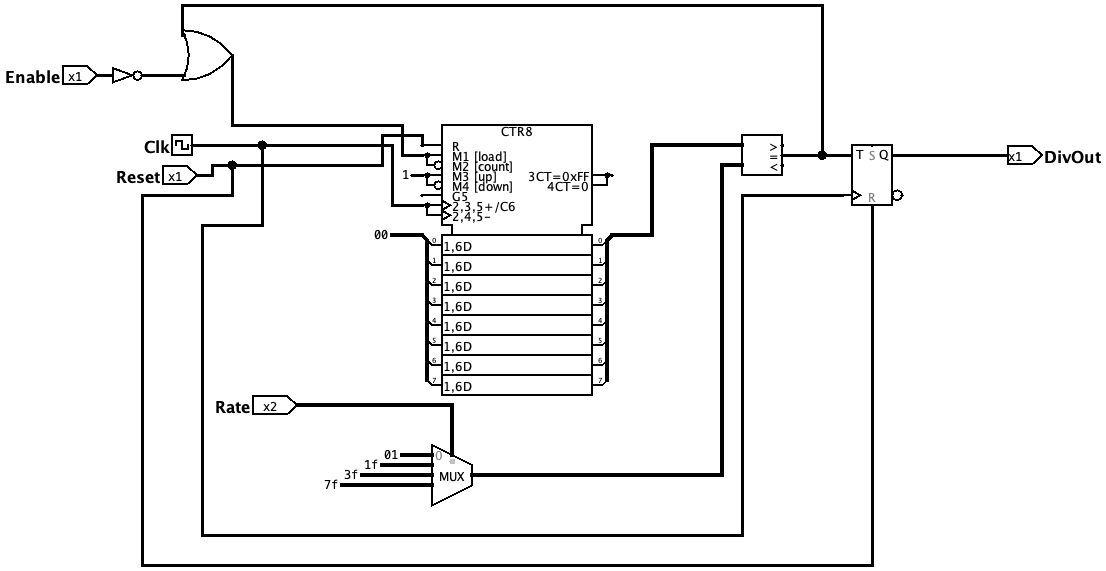
\includegraphics[width=0.65\textwidth]{lab5_rate_divider.png}
    \caption{A schematic of rate\_divider.}
    \label{f:rate_divider}
\end{figure}

\item Export the timing diagram as an image and include it in your report.

\begin{figure}[ht!]
    \centering
    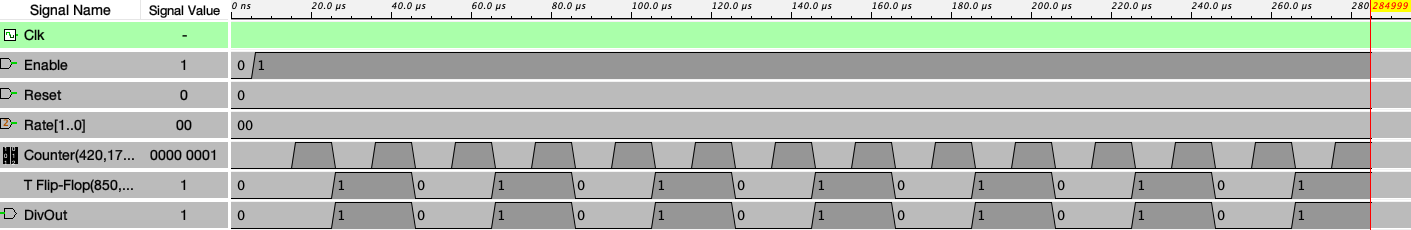
\includegraphics[width=0.65\textwidth]{lab5_timing_rate_divider.png}
    \caption{A timing simulation of rate\_divider.}
    \label{f:rate_divider_timing}
\end{figure}
\end{enumerate}

\section{Part III}

\begin{enumerate}
\item Fill in a table with your binary representation of each letter from S to Z.

\begin{table}[ht!]
\centering
\begin{tabular}{|c|l|c|} \hline
    \textbf{Letter} & \textbf{Morse Code} & \textbf{Pattern Representation (pattern length is 14 bits)} \\ \hline

    S & \textbf{$\bullet$ $\bullet$ $\bullet$} & 10101000000000\\ \hline
    T & \textbf{---} & 11100000000000 \\ \hline
    U & \textbf{$\bullet$ $\bullet$ --- } & 10101110000000 \\ \hline
    V & \textbf{$\bullet$ $\bullet$ $\bullet$ --- } & 10101011100000\\ \hline
    W & \textbf{$\bullet$ --- ---} & 10111011100000\\ \hline
    X & \textbf{--- $\bullet$ $\bullet$ ---} & 11101010111000\\ \hline
    Y & \textbf{--- $\bullet$ --- ---} & 11101011101110\\ \hline
    Z & \textbf{--- --- $\bullet$ $\bullet$} & 11101110101000\\ \hline

\end{tabular}
\caption{Morse Pattern Representation with fixed bit-width}
\label{tab:morse:pattern}
\end{table}

\item Export the subcircuit schematic as an image and include it in your report.

\begin{figure}[ht!]
    \centering
    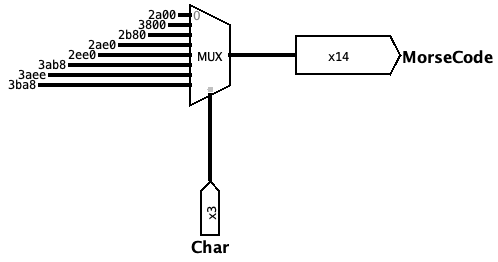
\includegraphics[width=0.65\textwidth]{lab5_morse_lut.png}
    \caption{A schematic of MORSE\_LUT.}
    \label{f:morse_lut}
\end{figure}
\end{enumerate}

\end{document}